% XCircuit output "ct_dsm_model.tex" for LaTeX input from ct_dsm_model.ps
\def\putbox#1#2#3{\makebox[0in][l]{\makebox[#1][l]{}\raisebox{\baselineskip}[0in][0in]{\raisebox{#2}[0in][0in]{#3}}}}
\def\rightbox#1{\makebox[0in][r]{#1}}
\def\centbox#1{\makebox[0in]{#1}}
\def\topbox#1{\raisebox{-\baselineskip}[0in][0in]{#1}}
\def\midbox#1{\raisebox{-0.5\baselineskip}[0in][0in]{#1}}
\begin{flushleft}
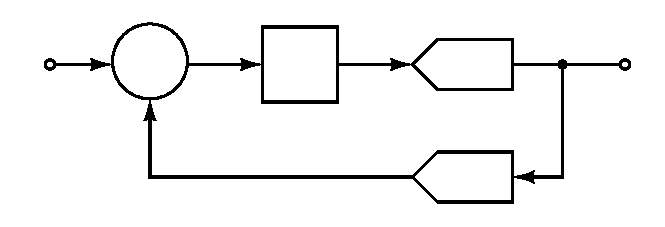
\epsfig{file=ct_dsm_model.ps}\\
% translate x=624 y=320 scale 0.38
\putbox{0.89in}{1.04in}{\centbox{\midbox{$\displaystyle\sum$}}}%
\putbox{3.93in}{1.10in}{$y(n)$}%
\putbox{0.06in}{1.10in}{$x(t)$}%
\putbox{1.89in}{1.01in}{\centbox{\midbox{$\displaystyle\int$}}}%
\putbox{0.76in}{0.70in}{\centbox{\midbox{$-$}}}%
\putbox{2.99in}{1.01in}{\centbox{\midbox{ADC}}}%
\putbox{2.99in}{0.24in}{\centbox{\midbox{DAC}}}%
\end{flushleft}
